\chapter{Ampelsystem}
\label{kapitel_ampelsystem}

\section{Allgemeines}

Das Ampelsystem ist ein Erinnerungs- und Best�tigungssystem welches beliebig f�r Studierende, LektorInnen und MitarbeiterInnen eingesetzt werden kann.
Hierbei werden dem Benutzer/der Benutzerin nach dem Login entsprechend offene Meldungen als rote bzw. gelbe Ampeln in der Titelleiste angezeigt (siehe Abbildung \ref{ampel_icons}).
Neue Meldungen k�nnen nur von Administratoren angelegt und gewartet werden.

\begin{figure}
	\centering
	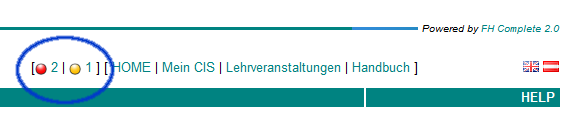
\includegraphics[width=0.70\textwidth]{CIS_Ampelsystem_Ampelicons.png}
	\caption{Offene Ampeln werden in der Titelleiste angezeigt}
	\label{ampel_icons}
\end{figure}

Nach dem Klicken auf eine offene Ampel wird eine �bersichtsseite geladen, auf der nun jede Meldung einzeln best�tigt werden kann (siehe Abbildung \ref{ampel_uebersicht}).
Eine Meldung kann dabei von folgenden Parametern eingeschr�nkt werden:

\begin{description}
	\item[Beschreibung:] Titel und Inhalt der Meldung.
	\item[Zielgruppe:] F�r eine Meldung kann genau definiert werden, wer diese angezeigt bekommen soll. Dies k�nnen definierte Personengruppen (MitarbeiterInnen, Studierende, ...) und/oder einzelne Personen sein.
	\item[Deadline:] Gibt an, ab wann das Datum einer Meldung als "`�berschritten"' gilt. Ab diesem Zeitpunkt, wird die Ampel auf "`rot"' gesetzt.
	\item[Vorlaufzeit (in Tagen):] Gibt an, ab wann die Meldung angezeigt und als "`gelb"' markiert wird.
	\item[Verfallzeit (in Tagen):] Gibt an, ab wann die Meldung nicht mehr angezeigt wird. Dabei spielt es keine Rolle, ob die Meldung best�tigt wurde oder nicht.
\end{description}

\begin{figure}
	\centering
	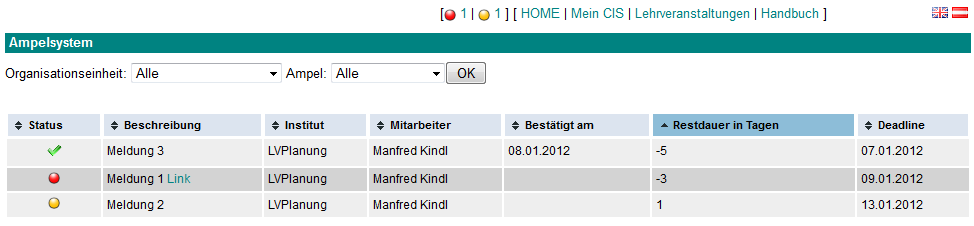
\includegraphics[width=1\textwidth]{CIS_Ampelsystem_Ampeluebersicht.png}
	\caption{�bersicht zum Best�tigen der Meldungen}
	\label{ampel_uebersicht}
\end{figure}

\section{Ampel�bersicht}
\label{ampeluebersicht}

Wie in Abbildung \ref{ampel_uebersicht} gezeigt, werden auf der �bersichtsseite alle Meldungen untereinander angef�hrt. Dabei werden Meldungen VOR der Deadline mit einer gelben Ampel gekennzeichnet, Meldungen, die die Deadline �berschritten haben, werden mit einer roten Ampel gekennzeichnet und best�tigte Meldungen werden mit einem gr�nen Haken markiert.
Wenn eine Meldung die Verfallszeit erreicht hat, wird diese nicht mehr angezeigt (Egal ob best�tigt oder nicht).

\subsection{Meldung best�tigen}

Klicken Sie in der letzten Spalte auf "`best�tigen"' um eine Meldung zu best�tigen. Daraufhin wird die Meldung mit einem gr�nen Haken markiert und bis zum Verfallsdatum als "`best�tigt"' angezeigt.

\section{Sonstiges}

Sie k�nnen die Liste durch Klicken auf die Spalten�berschriften sortieren.

\section{Ampel�bersicht f�r LeiterInnen}
\label{ampeluebersicht_leiterinnen}

Unter "`Mein CIS -> Ampel-�bersicht"' k�nnen Sie bei entsprechender Berechtigung den Status aller Meldungen einsehen.
Damit haben Sie einen �berblick, welche Personen eine entsprechende Meldung best�tigt haben oder nicht.
Sie k�nnen die Liste nach Organisationseinheit und/oder Bezeichnung der Ampel filtern und durch Klicken auf die Spalten�berschrift sortieren.

In der Spalte "`Best�tigt am"' ist ersichtlich, wann die Meldung best�tigt wurde.
Die Spalte "`Restdauer in Tagen"' gibt an, wann die Deadline der Meldung erreicht wird bzw. bei negativen Zahlen, um wieviele Tage die Deadline �berschritten wurde.